\documentclass[11pt,a4paper,oneside]{report}
\usepackage{helvetica}
\usepackage{tikz}
\usepackage{pgf-umlcd}

\begin{document}

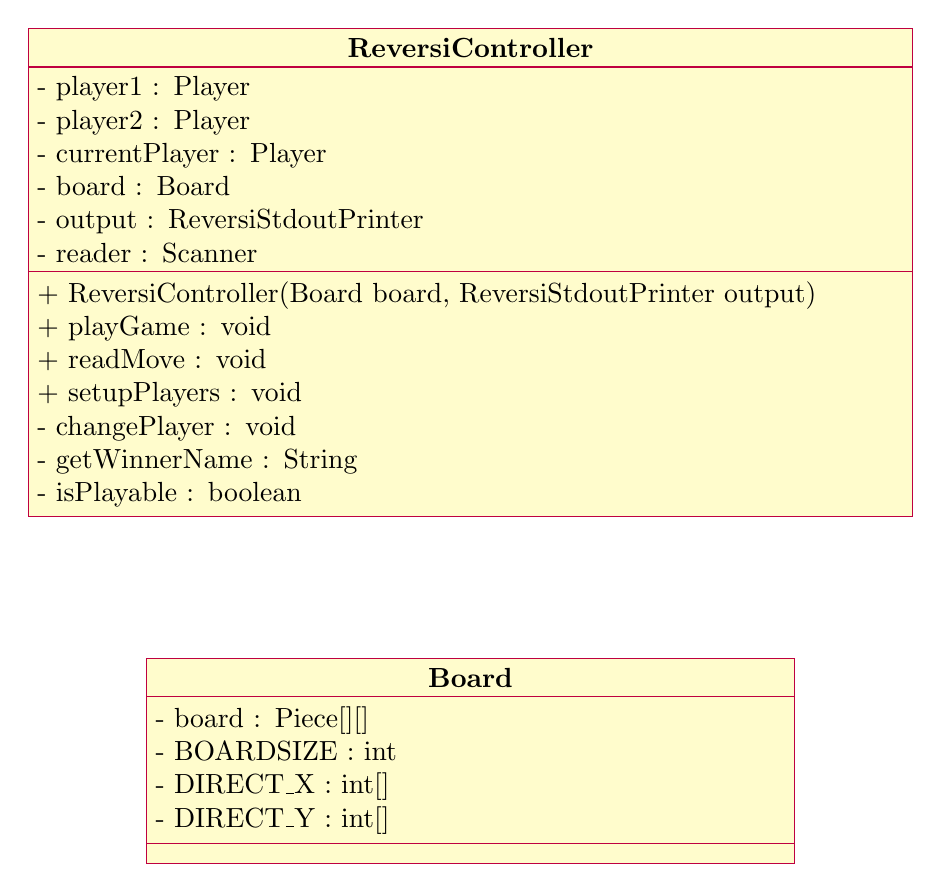
\begin{tikzpicture}
\begin{class}[text width=11cm]{ReversiController}{0,8} 
\attribute{- player1 : Player}
\attribute{- player2 : Player}
\attribute{- currentPlayer : Player}
\attribute{- board : Board}
\attribute{- output : ReversiStdoutPrinter }
\attribute{- reader : Scanner }
\operation{+ ReversiController(Board board, ReversiStdoutPrinter output)} 
\operation{+ playGame : void}
\operation{+ readMove : void}
\operation{+ setupPlayers : void}
\operation{- changePlayer : void}
\operation{- getWinnerName : String}
\operation{- isPlayable : boolean}
\end{class}

\begin{class}[text width=8cm]{Board}{0,0}
\attribute{- board : Piece[][]}
\attribute{- BOARDSIZE : int}
\attribute{- DIRECT\_X : int[]}
\attribute{- DIRECT\_Y : int[]}
\end{class}

\end{tikzpicture}

\end{document}
